\documentclass{article}

\usepackage{amssymb,amsmath,amsfonts,amstext}
\usepackage{graphicx}
%\usepackage{subfigure}
\usepackage{mathtools}
\usepackage{stmaryrd}
\usepackage{color}
\usepackage{verbatim}
\usepackage{amsthm}
\usepackage{esint}
\usepackage{caption,subcaption}
\usepackage{titlesec}
\setcounter{secnumdepth}{4}
\usepackage{geometry}
\geometry{left=3.18cm,right=3.18cm,top=2.54cm,bottom=2.54cm}


\title{ODE solver by neural network}
\author{Xiaoguai Li}
\date{}

\begin{document}


\maketitle

\section{Goal}
Train a deep neural network by TensorFlow with two hidden layers, 50 neurons per layer, and a hyperbolic tangent activation function to solve ODE
\begin{equation}\nonumber
\frac{\partial^2 u}{\partial x^2} - u = -(\pi^2+1)\sin(\pi x)
\end{equation}
with boundary conditions $u(-1)=u(1)=0$.
Check convergence of number of training points. Plot the approximation error in the L2 norm as the number of training points is increased.

\section{Results}
The following figures are directly generated by NN\_ODE.py, which is the main script. It imports NeuralNetwork from PDEsolver\_tf.py. At the beginning of NN\_ODE.py, number of training data can be defined.
1000 test data is used. 40000 iteration is used to train the model. Batch size is full. Fig.1
shows the error of prediction with respect to different numbers of training points. This plot shows
convergence.

\begin{figure}[htbp]
\center
    \begin{subfigure}{0.45\textwidth}
        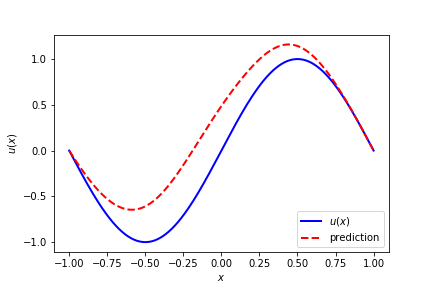
\includegraphics[width=\textwidth]{figures/3TrainingPoints}
        \caption{3 Training Points}
    \end{subfigure}
    ~ %add desired spacing between images, e. g. ~, \quad, \qquad, \hfill etc. 
      %(or a blank line to force the subfigure onto a new line)
    \begin{subfigure}{0.45\textwidth}
        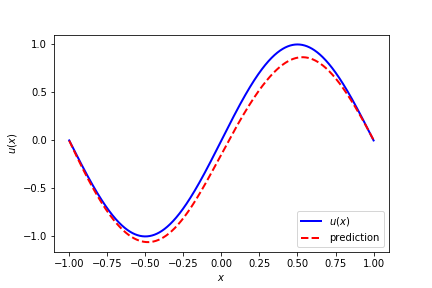
\includegraphics[width=\textwidth]{figures/6TrainingPoints}
        \caption{6 Training Points}
    \end{subfigure}
        ~ %add desired spacing between images, e. g. ~, \quad, \qquad, \hfill etc. 
      %(or a blank line to force the subfigure onto a new line)
    \begin{subfigure}{0.45\textwidth}
        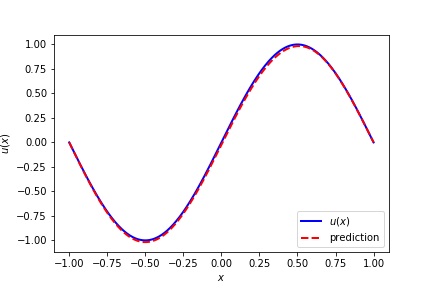
\includegraphics[width=\textwidth]{figures/9TrainingPoints}
        \caption{9 Training Points}
    \end{subfigure}
~ %add desired spacing between images, e. g. ~, \quad, \qquad, \hfill etc. 
      %(or a blank line to force the subfigure onto a new line)
    \begin{subfigure}{0.45\textwidth}
        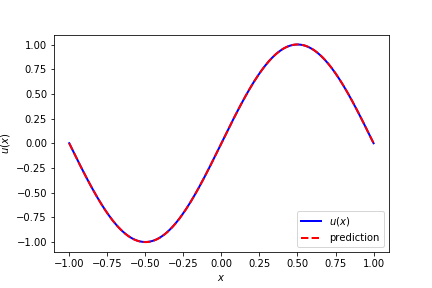
\includegraphics[width=\textwidth]{figures/12TrainingPoints}
        \caption{12 Training Points}
    \end{subfigure}
\end{figure}

     \addtocounter{figure}{-1}  
\begin{figure}[htbp]
\center

    \begin{subfigure}{0.45\textwidth}
        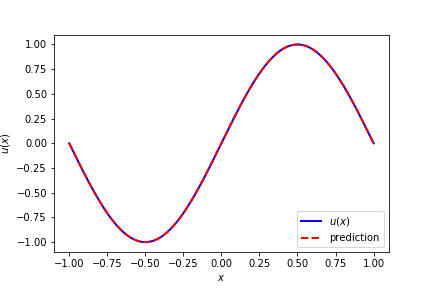
\includegraphics[width=\textwidth]{figures/15TrainingPoints}
           \addtocounter{subfigure}{4}  
        \caption{15 Training Points}
    \end{subfigure}
        ~ %add desired spacing between images, e. g. ~, \quad, \qquad, \hfill etc. 
      %(or a blank line to force the subfigure onto a new line)
    \begin{subfigure}{0.45\textwidth}
        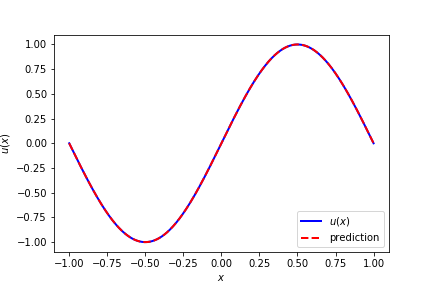
\includegraphics[width=\textwidth]{figures/18TrainingPoints}
        \caption{18 Training Points}
    \end{subfigure}
~ %add desired spacing between images, e. g. ~, \quad, \qquad, \hfill etc. 
      %(or a blank line to force the subfigure onto a new line)
    \begin{subfigure}{0.45\textwidth}
        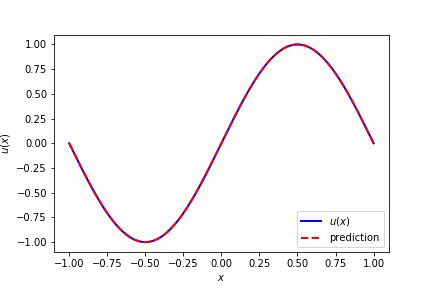
\includegraphics[width=\textwidth]{figures/21TrainingPoints}
        \caption{21 Training Points}
    \end{subfigure}
        ~ %add desired spacing between images, e. g. ~, \quad, \qquad, \hfill etc. 
      %(or a blank line to force the subfigure onto a new line)
    \begin{subfigure}{0.45\textwidth}
        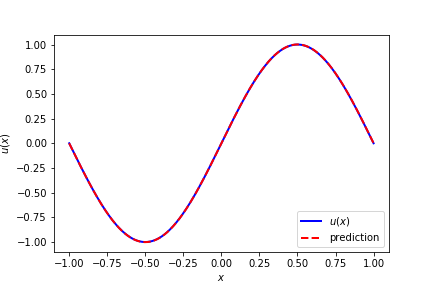
\includegraphics[width=\textwidth]{figures/24TrainingPoints}
        \caption{24 Training Points}
    \end{subfigure}
~ %add desired spacing between images, e. g. ~, \quad, \qquad, \hfill etc. 
      %(or a blank line to force the subfigure onto a new line)
    \begin{subfigure}{0.45\textwidth}
        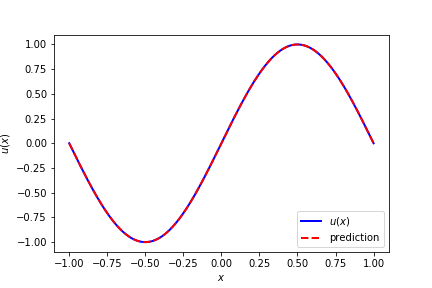
\includegraphics[width=\textwidth]{figures/27TrainingPoints}
        \caption{27 Training Points}
    \end{subfigure}
        ~ %add desired spacing between images, e. g. ~, \quad, \qquad, \hfill etc. 
      %(or a blank line to force the subfigure onto a new line)
    \begin{subfigure}{0.45\textwidth}
        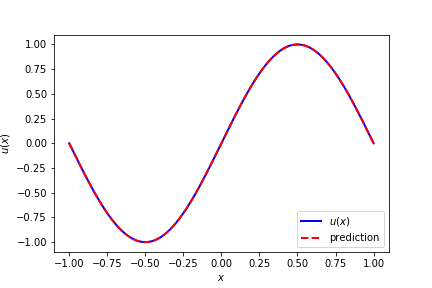
\includegraphics[width=\textwidth]{figures/30TrainingPoints}
        \caption{30 Training Points}
    \end{subfigure}
    \caption{Prediction results with different numbers of training data}

\end{figure}

\begin{figure}
    \center
    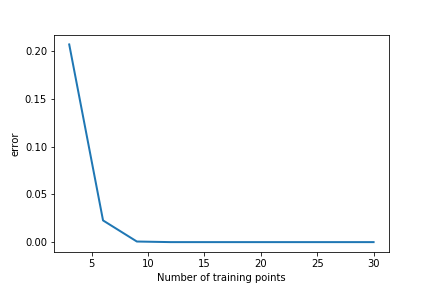
\includegraphics[width=0.6\textwidth]{figures/error.png}
    \caption{Prediction error decreases with increasing number of training data}
\end{figure}


\end{document}



